\documentclass[11pt]{article}
\renewcommand{\baselinestretch}{1.15}

% some commonly used packages are included here
\usepackage[utf8]{inputenc}
\usepackage{graphicx}
\usepackage{float}
\usepackage{multirow}
\usepackage[table,xcdraw]{xcolor}
\usepackage{listings}
\usepackage[a4paper, total={6.3in, 9.4in}]{geometry}
\usepackage{color}
\usepackage{booktabs}
\usepackage{tabularx}
\usepackage{amssymb}
\usepackage{vhistory}

% some configurations for the listings package
\definecolor{codegreen}{rgb}{0,0.6,0}
\definecolor{codegray}{rgb}{0.5,0.5,0.5}
\definecolor{codepurple}{rgb}{0.58,0,0.82}
\definecolor{backcolour}{rgb}{0.95,0.95,0.92}
\lstdefinestyle{mystyle}{
    backgroundcolor=\color{backcolour},
    commentstyle=\color{codegreen},
    keywordstyle=\color{magenta},
    numberstyle=\tiny\color{codegray},
    stringstyle=\color{codepurple},
    basicstyle=\footnotesize\ttfamily,
    breakatwhitespace=false,
    breaklines=true,
    captionpos=b,
    keepspaces=true,
    numbers=left,
    numbersep=5pt,
    showspaces=false,
    showstringspaces=false,
    showtabs=false,
}
\lstset{style=mystyle}

% beginning of the report
\begin{document}
\begin{titlepage}
\begin{center}

% school logo

\includegraphics[width=0.9\textwidth]{images/ntu_logo.png}
\\[5cm]

% project title
\uppercase{\textbf{NTU HPC Cluster User Guide}}
\\[5cm]

% submited by ...
\uppercase{
\textbf{
%Liu Siyuan (SLIU019@e.ntu.edu.sg)
}}

\vfill

% Bottom of the page
\textsc{\bfseries NTU HPC Team}
\\
\textbf{https://ntuhpc.org}

\end{center}
\end{titlepage}

\begin{versionhistory}
  \vhEntry{1.0}{27/02/2017}{Liu Siyuan}{created}
  \vhEntry{1.1}{07/03/2017}{Liu Siyuan}{update cluster address, add monitoring information}
  \vhEntry{1.2}{22/03/2017}{Liu Siyuan}{add OS and package information}
\end{versionhistory}
\newpage
\pagenumbering{gobble}
\tableofcontents
\newpage
\pagenumbering{arabic}
% add your contents here
\section{Overview}

The NTU HPC cluster, located at Parallel and Distributed System Lab (PDSL), is managed and used by the NTU HPC team\footnote{http://ntuhpc.org}. Its main purpose is for members of NTU HPC to get hands-on skills on optimizing applications for supercomputers and practice applications used in student cluster competitions.

\subsection{Cluster architecture}

The cluster consists of 4 nodes. There are 2 CPU nodes and 2 GPU nodes. The nodes are connected with 1Gbit/s Ethernet. Amongs the nodes, only compute0 is connected to NTU's network. The detailed specification for both CPU and GPU nodes are shown in Table \ref{table:cpu} and Table \ref{table:gpu}.

\begin{table}[ht]
\centering
\caption{CPU node specification}
\label{table:cpu}
\begin{tabular}{|l|l|}
\hline
\textbf{Nodes}      & compute0, compute1                       \\ \hline
\textbf{CPU}        & Intel X5660 (6 cores, 2.8GHz, HT, Turbo) x 2 \\ \hline
\textbf{Memory}     & DDR3 32GB                                \\ \hline
\textbf{Hard drive} & 480GB SATA HDD                           \\ \hline
\textbf{Network}    & 1Gbit/s Ethernet                         \\ \hline
\end{tabular}
\end{table}

\begin{table}[ht]
\centering
\caption{GPU node specification}
\label{table:gpu}
\begin{tabular}{|l|l|}
\hline
\textbf{Nodes}      & compute2, compute3                             \\ \hline
\textbf{CPU}        & Intel E5-2695 v2 (12 cores, 2.4GHz, HT, Turbo) x 2 \\ \hline
\textbf{GPU}        & NVIDIA Tesla P100 (PCIE-16GB)                  \\ \hline
\textbf{Memory}     & DDR3 48GB                                      \\ \hline
\textbf{Hard drive} & 480GB SATA HDD                                 \\ \hline
\textbf{Network}    & 1Gbit/s Ethernet                               \\ \hline
\end{tabular}
\end{table}

\noindent The architecture of the NTU HPC cluster is shown in Figure \ref{fig:arch}.

\begin{figure}[ht]
    \centering
    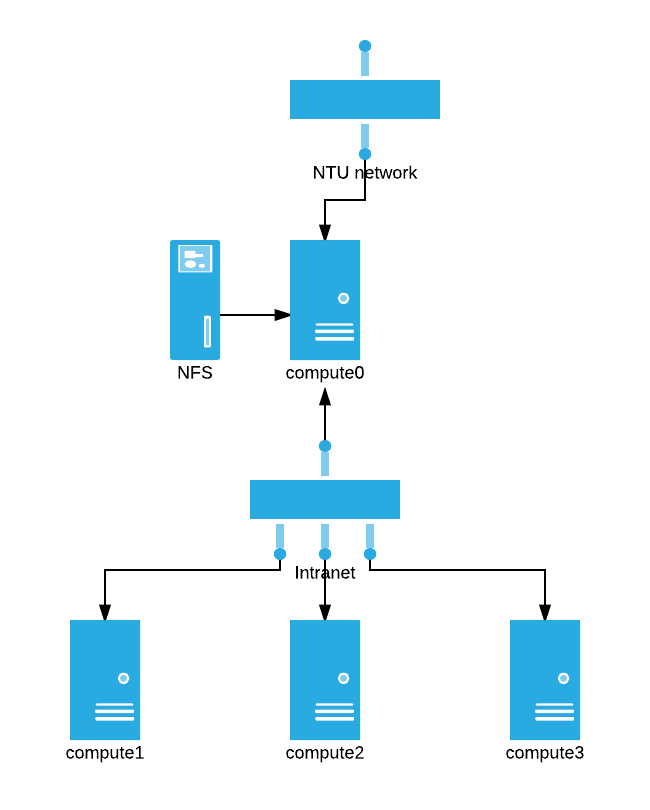
\includegraphics[width=0.55\textwidth]{images/arch.png}
    \caption{NTU HPC cluster architecture}
    \label{fig:arch}
\end{figure}
\section{Accessing the cluster}

The cluster is located at Parallel and Distributed System Lab (PDSL), School of Computer Science and Engineering. Among the cluster nodes, compute0 serves as the login node for users to login to the system. To login, connect to the server at cluster.ntuhpc.org with SSH. For example

\begin{lstlisting}
$ ssh <username>@cluster.ntuhpc.org
\end{lstlisting}

\noindent After logging in, all cluster nodes can be access with SSH. For example

\begin{lstlisting}
$ ssh <username>@<nodename>
\end{lstlisting}

\noindent Currently, the cluster has the following nodes

\begin{itemize}
    \item compute0
    \item compute1
    \item compute2
    \item compute3
\end{itemize}

\subsection{Changing password}

Upon successful login, it's the user's responsibility to change his/her password. To change password

\begin{lstlisting}
$ yppasswd
\end{lstlisting}

\subsection{Changing shell}

By default, your login shell is BASH. If you prefer to use other shell, change the shell with

\begin{lstlisting}
$ ypchsh -s /path/to/your/shell
\end{lstlisting}

\noindent For example, to change default shell to ZSH

\begin{lstlisting}
$ ypchsh -s /bin/zsh
\end{lstlisting}
\section{Data storage}

To support data sharing among multiple cluster nodes for running dsitributed applications, a Network File System (NFS) has been setup. Currently, the following folders are shared across all cluster nodes

\begin{itemize}
    \item /opt (for sharing software packages, etc.)
    \item /home (for sharing user data)
\end{itemize}

\noindent If you are working on your own, you could store all data in your home directory \lstinline{/home/<username>}. If you are collaborating with others on an application, contact the administrators to create a folder in \lstinline{/home/public} which could be shared among multiple users.
\section{Compiling application}

The NTU HPC cluster employs the Lmod system to manage the compilers and libraries. This system allows users to easily load a package, switch between different versions of a package, and unload a package. These features are implemented by smartly changing user's environment variables (e.g. \lstinline{PATH}, and \lstinline{LD_LIBRARY_PATH}) under the hood. The changes are only effective for users' current session. A list of packages available on the cluster in presented in Appendix \ref{packages}.

\subsection{Basic Lmod commands}

To check what are the available packages, use

\begin{lstlisting}
$ module av
\end{lstlisting}

\noindent To load a package, use

\begin{lstlisting}
$ module load <packagename>
\end{lstlisting}

\noindent The above command will load the default version for that package (marked with \lstinline{(D)}), to load a specific version, use

\begin{lstlisting}
$ module load <packagename>/<version>
\end{lstlisting}

\noindent To switch the version of a package after it has been loaded, use the above command with the version you want. To check what modules are loaded, use

\begin{lstlisting}
$ module list
\end{lstlisting}

\noindent To unload a module after use, use

\begin{lstlisting}
$ module unload <packagename>
\end{lstlisting}

\noindent To unload all loaded modules at once, use

\begin{lstlisting}
$ module purge
\end{lstlisting}
\section{Submitting jobs}

To be added.
\section{Cluster monitoring}

The NTU HPC cluster uses Ganglia to collect metrics for monitoring purposes. It also has a Grafana dashboard as frontend for metric visualization. The dashboard can be accessed at http://grafana.ntuhpc.org anonymously. On the site, please select the dashboard \textit{NTU HPC cluster}. By default, the dashboard shows metrics for all nodes in the cluster. To display metrics for a single node, you can change the \textit{node} variable at the top left corner.
\newpage
\appendix

\section{Available packages} \label{packages}

\begin{table}[H]
\centering
\label{table:packages}
\begin{tabular}{|l|l|l|}
\hline
\rowcolor[HTML]{FCFF2F} 
\textbf{Package} & \textbf{Description} & \textbf{Category}                \\ \hline
GCC 4.9.4        &                      &                                  \\ \cline{1-2}
GCC 5.4.0        &                      &                                  \\ \cline{1-2}
GCC 6.3.0        &                      & \multirow{-3}{*}{Compilers}      \\ \hline
OpenMPI 1.10.3   &                      &                                  \\ \cline{1-2}
OpenMPI 2.0.2    &                      & \multirow{-2}{*}{MPI}            \\ \hline
FFTW 3.3.4       &                      &                                  \\ \cline{1-2}
OpenBLAS 0.2.18  &                      &                                  \\ \cline{1-2}
ScaLAPACK 2.0.2  &                      & \multirow{-3}{*}{Math libraries} \\ \hline
CUDA 8.0.44      &                      & CUDA                             \\ \hline
Python 2.7.12    &                      & Programming languages            \\ \hline
protobuf 3.2.0   &                      & Common libraries                 \\ \hline
CMake 3.7.1      &                      & Utilities                        \\ \hline
\end{tabular}
\end{table}

\end{document}
